\section{Results}

Table \ref{tab:fluid_comparison} shows a summary of the comparison of the five fluid simulation methods.

\begin{table}[!htbp]
\centering
\caption{Comparison of Fluid Simulation Methods}
\label{tab:fluid_comparison}
\begin{tabularx}{\columnwidth}{l X X}
\toprule
\textbf{Method} & \textbf{Pro} & \textbf{Con} \\
\midrule
Grid&
Fast (real-time) \newline
Unconditionally stable &
Loss of detail \newline
Not physically accurate \\
\midrule
Particle&
Fast &
Limitation of input particle position \newline
Particle collapse \\
\midrule
PIC&
Stable &
High numerical dissipation \newline
Particles lose energy quickly \\
\midrule
PIC/FLIP &
More realistic and dynamic motion &
Less stable \newline
Needs tuning \\
\midrule
APIC &
Preserves rotation &
More complex \newline
Slower \\
\bottomrule
\end{tabularx}
\end{table}

\subsection{Grid}

We evaluated the performance of the Grid method with a 50x50 grid. Figure~\ref{fig:grid} shows simulation snapshots of the grid simulation.

The grid-based method is easy to use and stable. It works well for smooth and slow fluid motion. But it also has some limits. Small details like sharp edges are often lost because values are spread out too much. It can also look blurry over time. Since the grid is fixed, it is harder to follow fast-moving or thin parts of the fluid. Overall, it is simple and works well for basic fluid scenes, but not good for effects that need high detail.

\begin{figure*}[h]
    \centering
    \begin{subfigure}[b]{0.2\textwidth}
        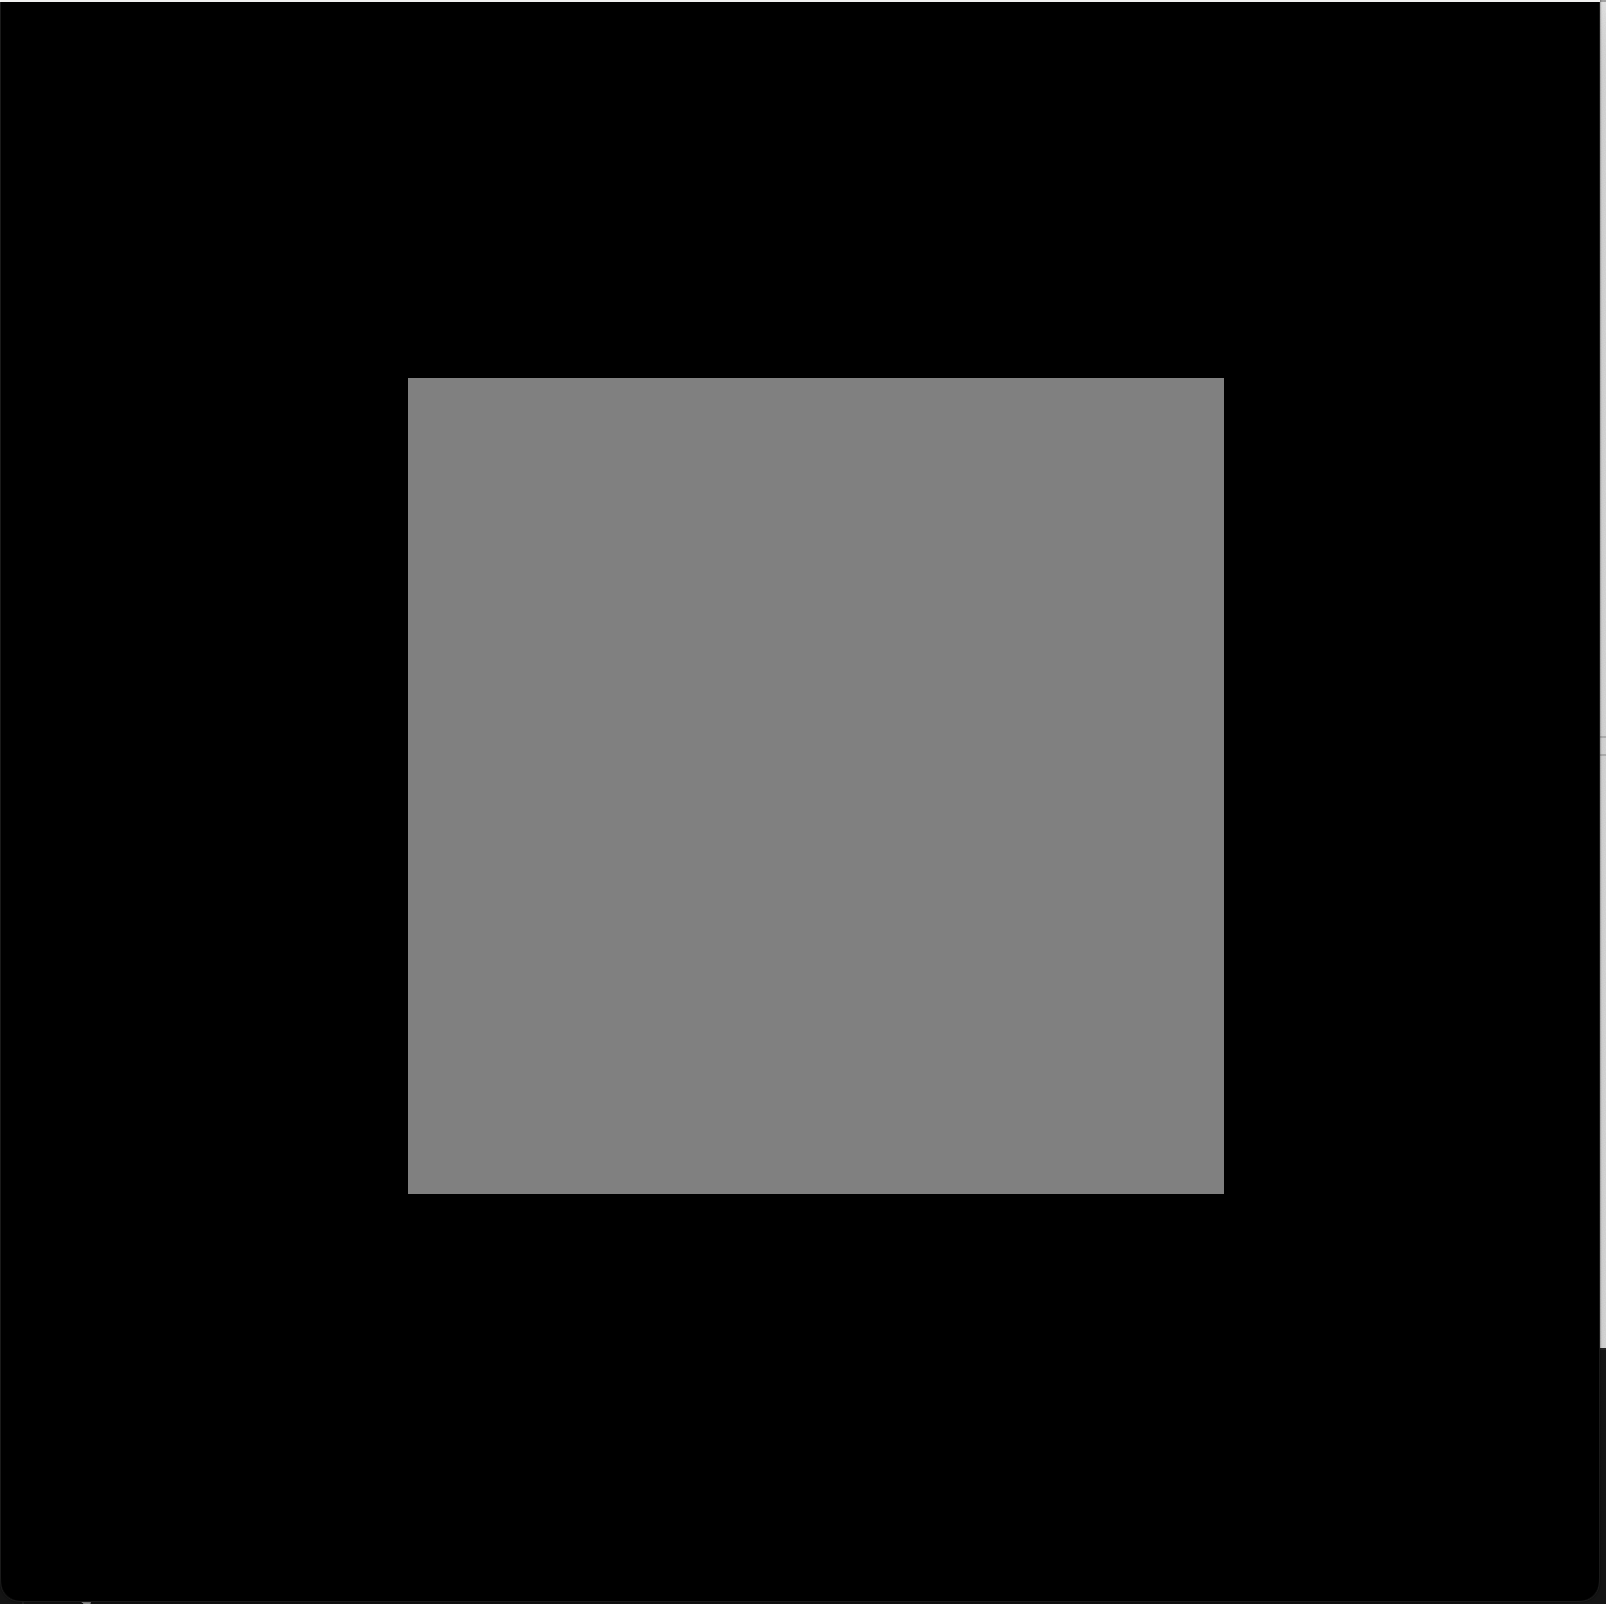
\includegraphics[width=\textwidth]{figures/grid50_init.png}
        \caption{initialization}
    \end{subfigure}
    \hspace{1em}
    \begin{subfigure}[b]{0.2\textwidth}
        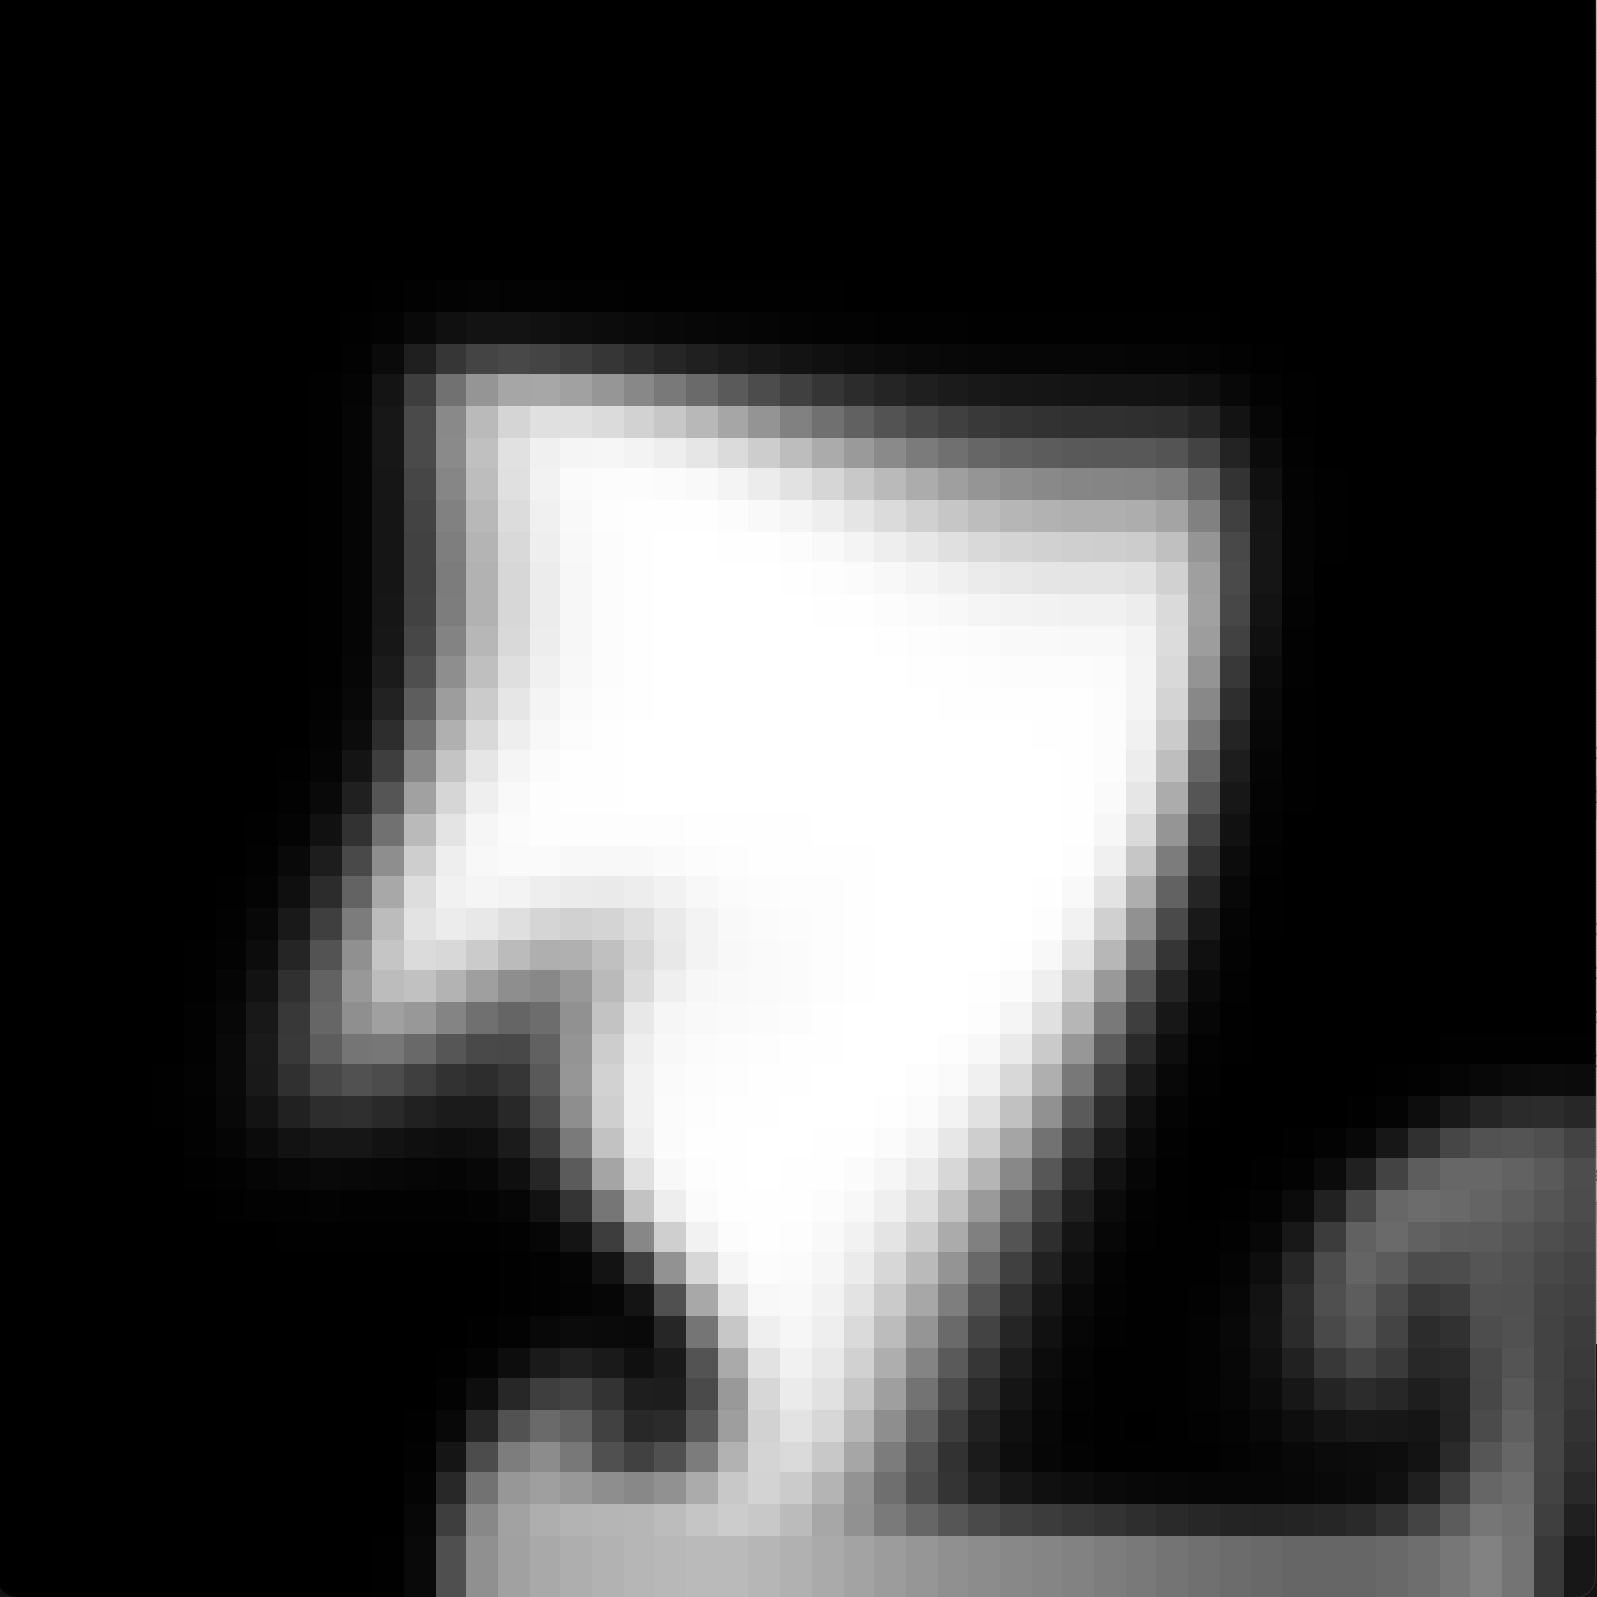
\includegraphics[width=\textwidth]{figures/grid50_1.png}
        \caption{first stage}
    \end{subfigure}
    \hspace{1em}
    \begin{subfigure}[b]{0.2\textwidth}
        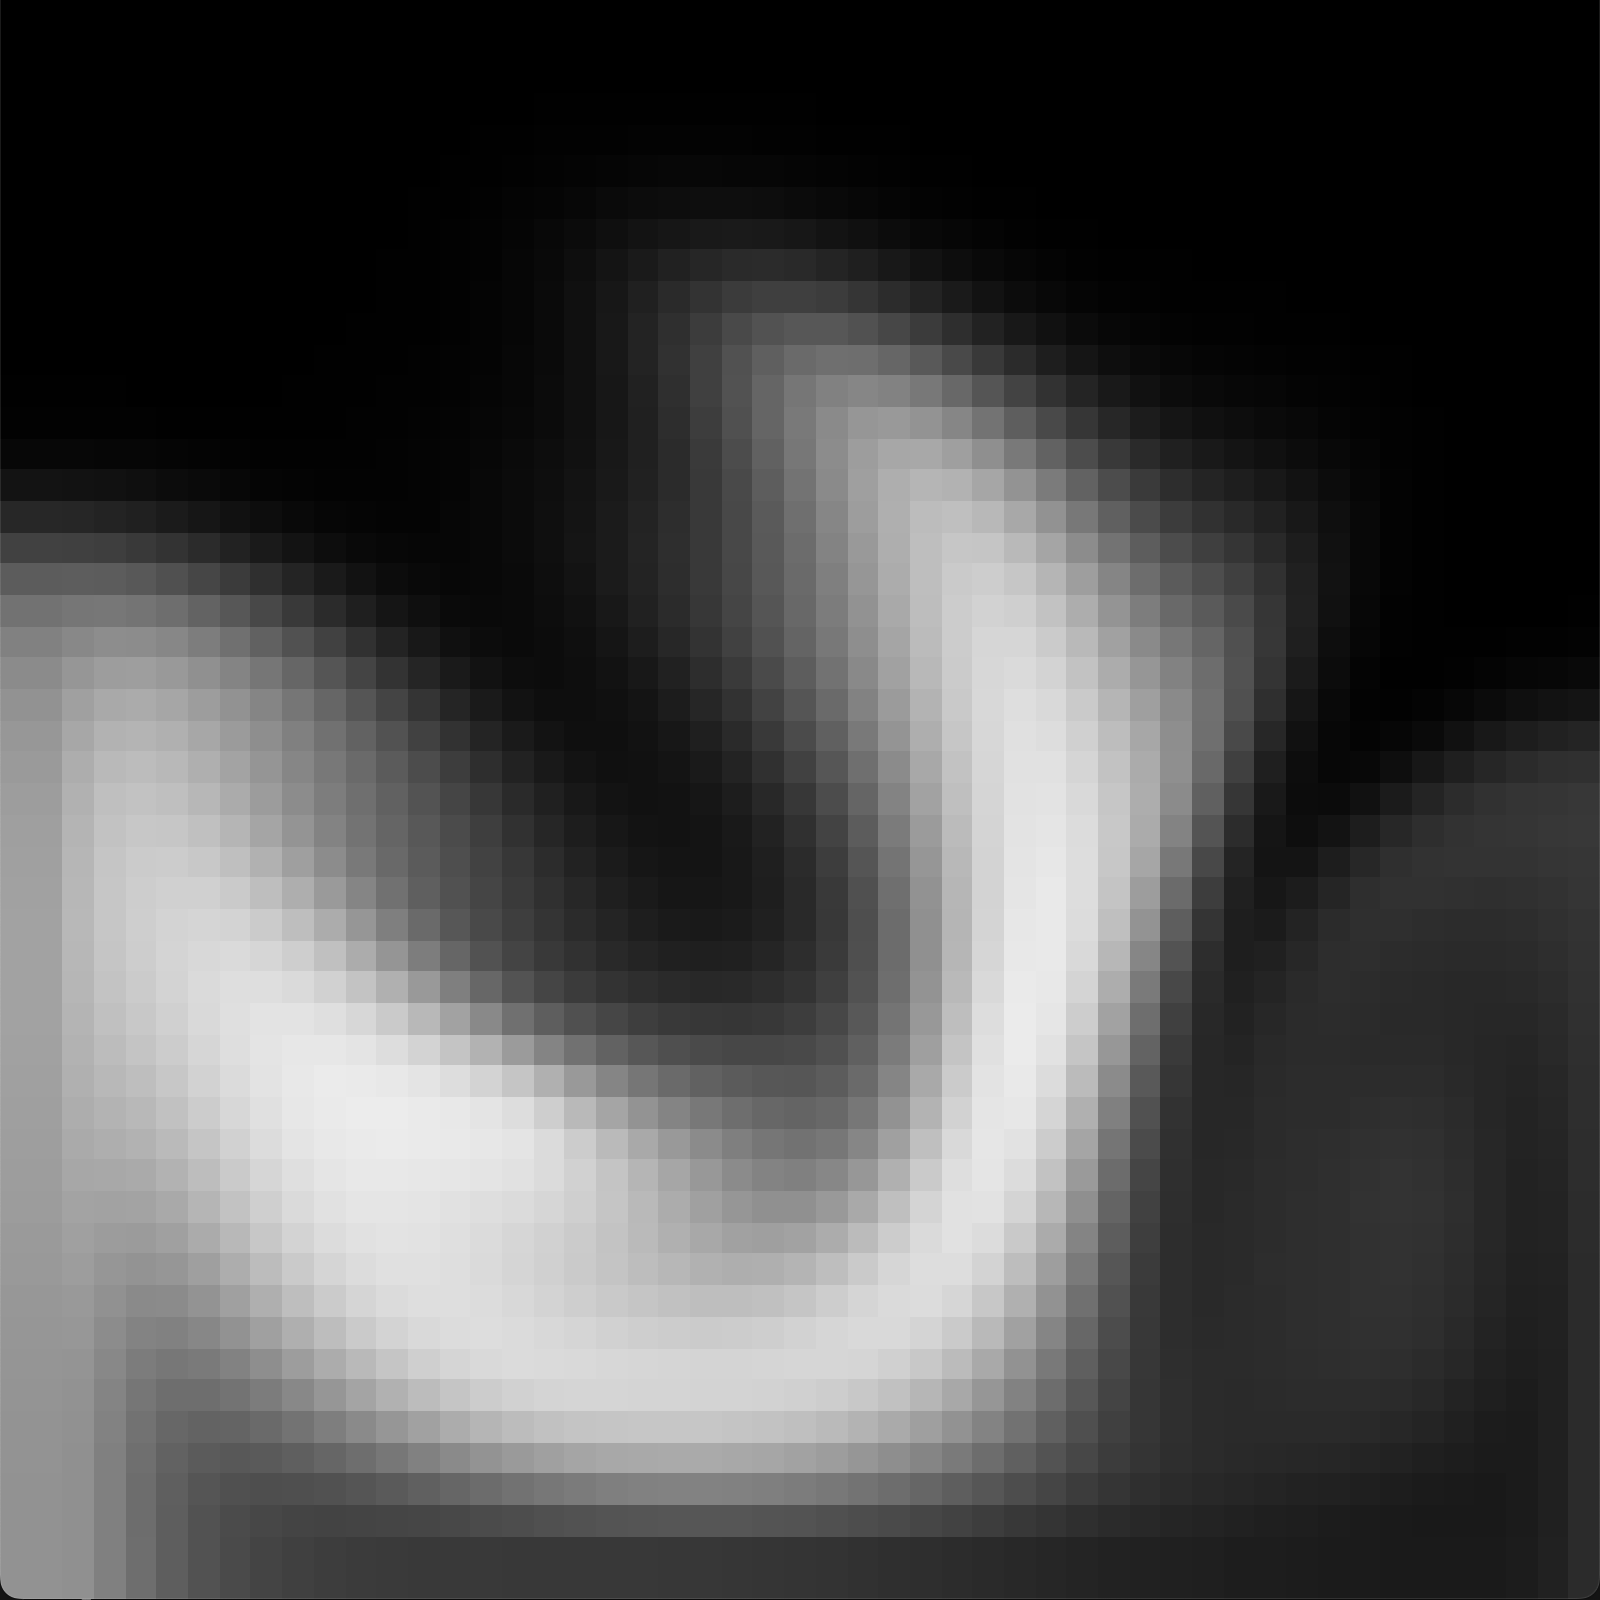
\includegraphics[width=\textwidth]{figures/grid50_2.png}
        \caption{second stage}
    \end{subfigure}
    \hspace{1em}
    \begin{subfigure}[b]{0.2\textwidth}
        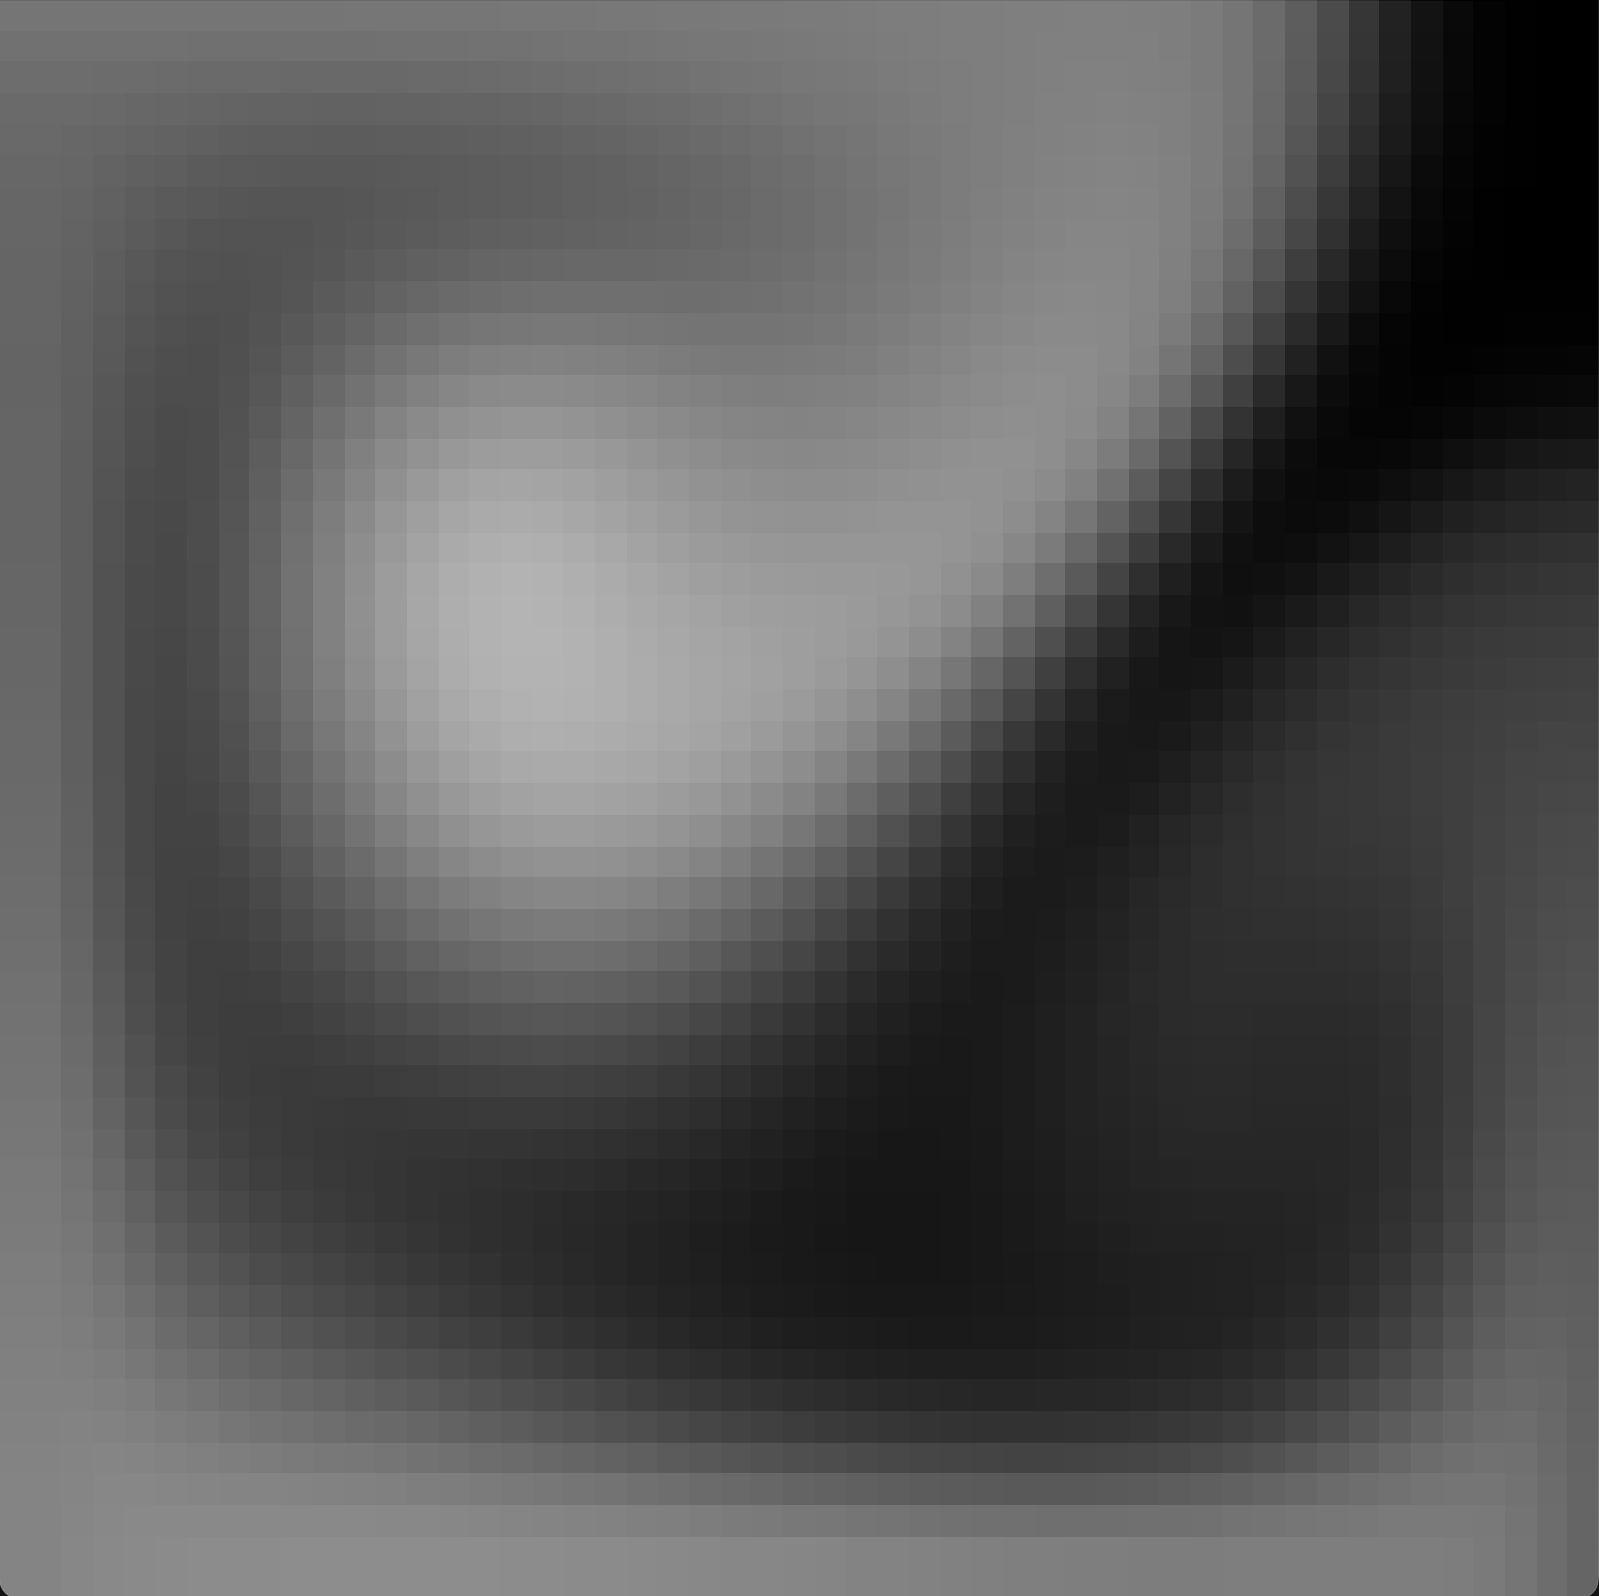
\includegraphics[width=\textwidth]{figures/grid50_3.png}
        \caption{third stage}
    \end{subfigure}
    \caption{Stages of Stable Fluids simulation 
    (a) shows the initial grid configuration
    (b)–(d) show different stages of the simulation}
    \label{fig:grid}
\end{figure*}

\subsection{Particle}
Smoothed Particle Hydrodynamics (SPH) contributed to a fast and scalable fluid simulation. The method is more intuitive, and can be used to model free surfaces, avoiding issues that are present in grid simulation such as grid aliasing.
Compared to Stable Fluids, SPH is less stable, and can lead to particle clumping if not stabilized. When initializing the particles, the method is sensitive to particle distribution and requires attention to tuning the smoothing kernels. Figure~\ref{fig:sph} shows the SPH simulation with 400 particles. It handles free surfaces naturally, but can become unstable and prone to clumping over time.

\begin{figure*}[h]
    \centering
    \begin{subfigure}[b]{0.2\textwidth}
        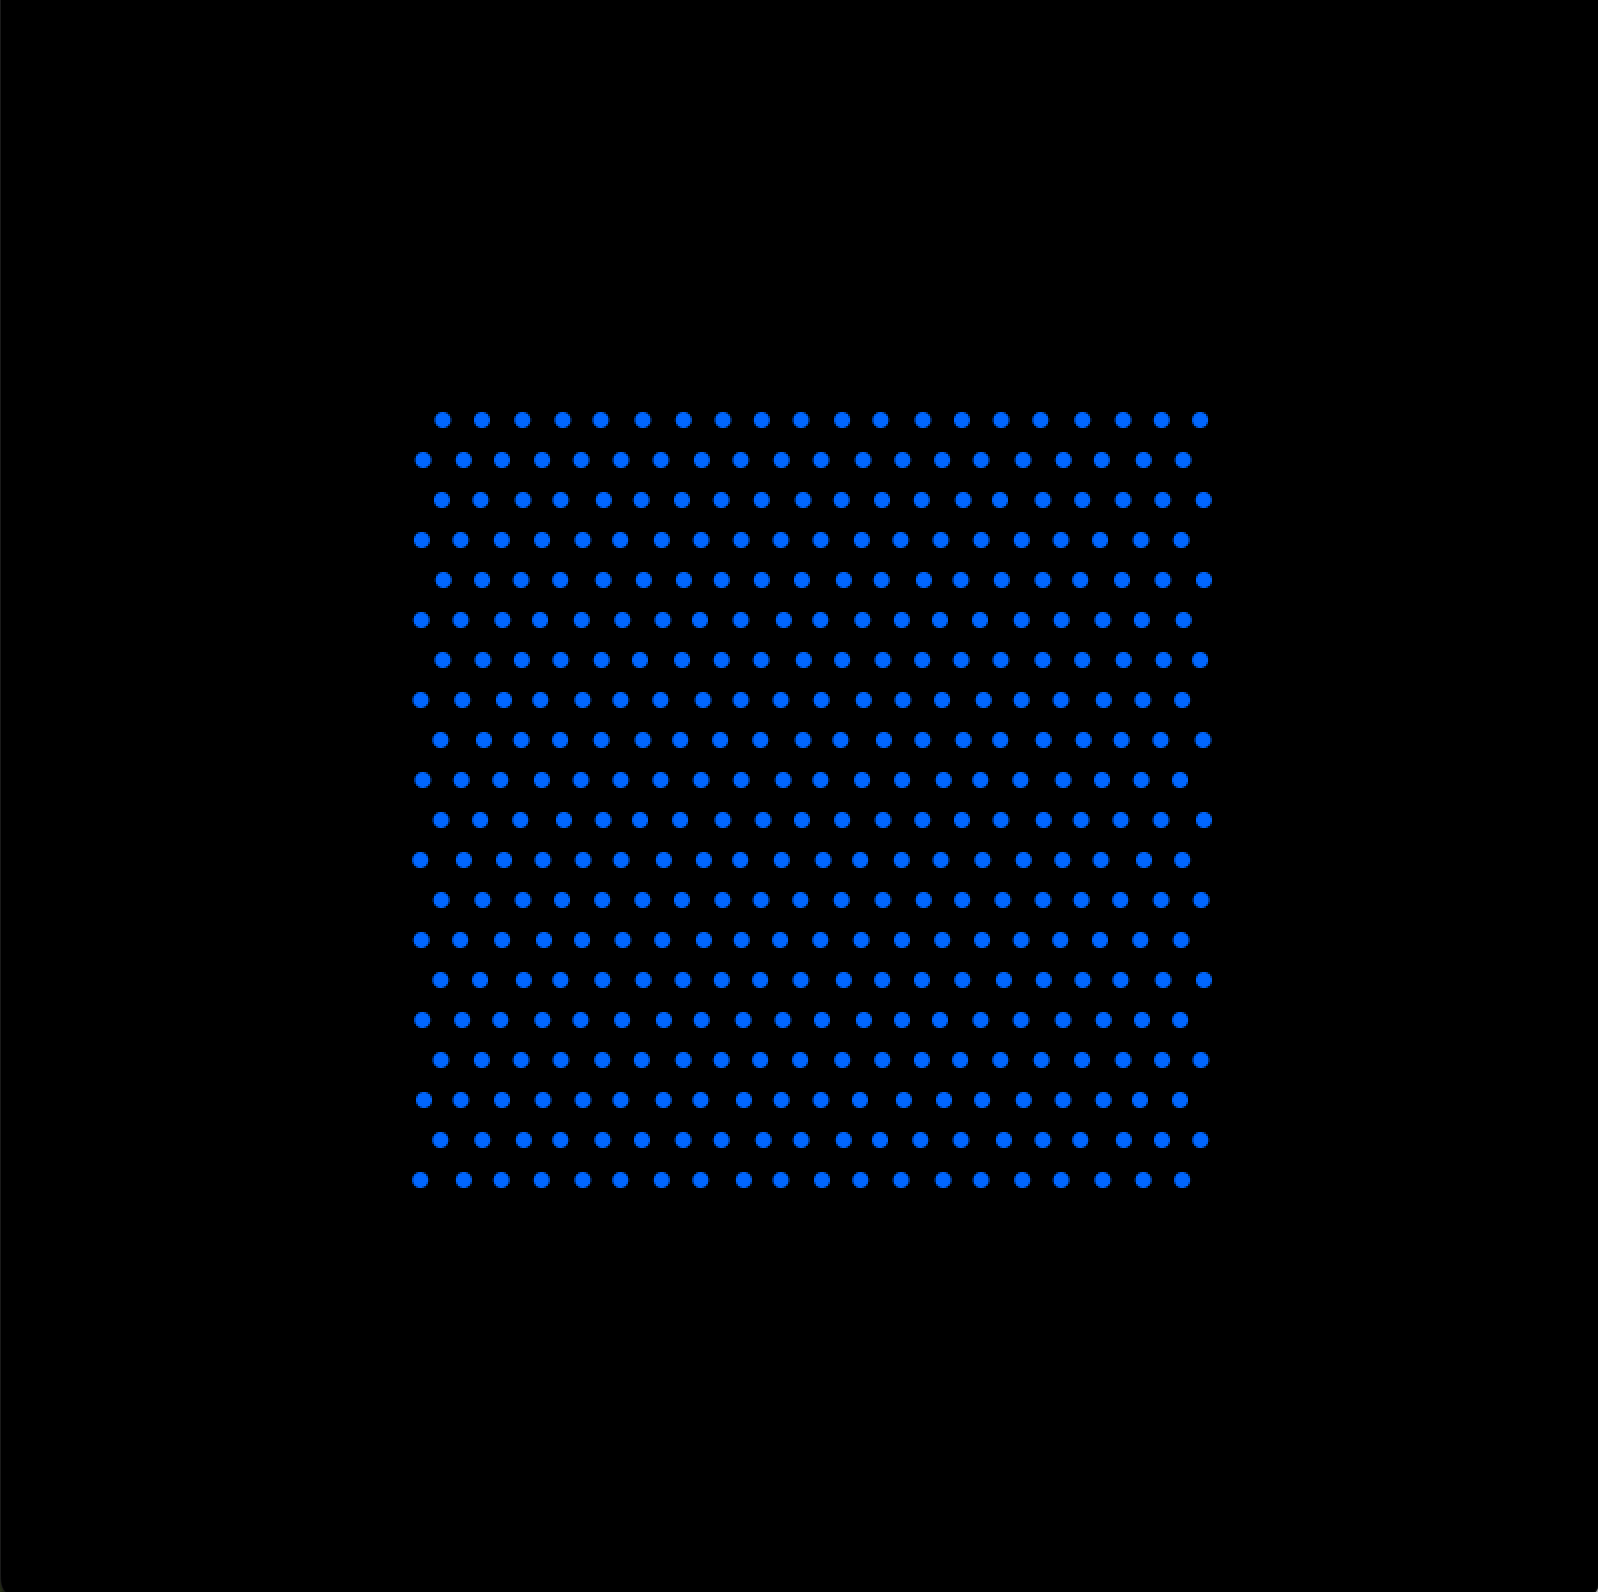
\includegraphics[width=\textwidth]{figures/particle400_1.png}
        \caption{initialization}
    \end{subfigure}
    \hspace{1em}
    \begin{subfigure}[b]{0.2\textwidth}
        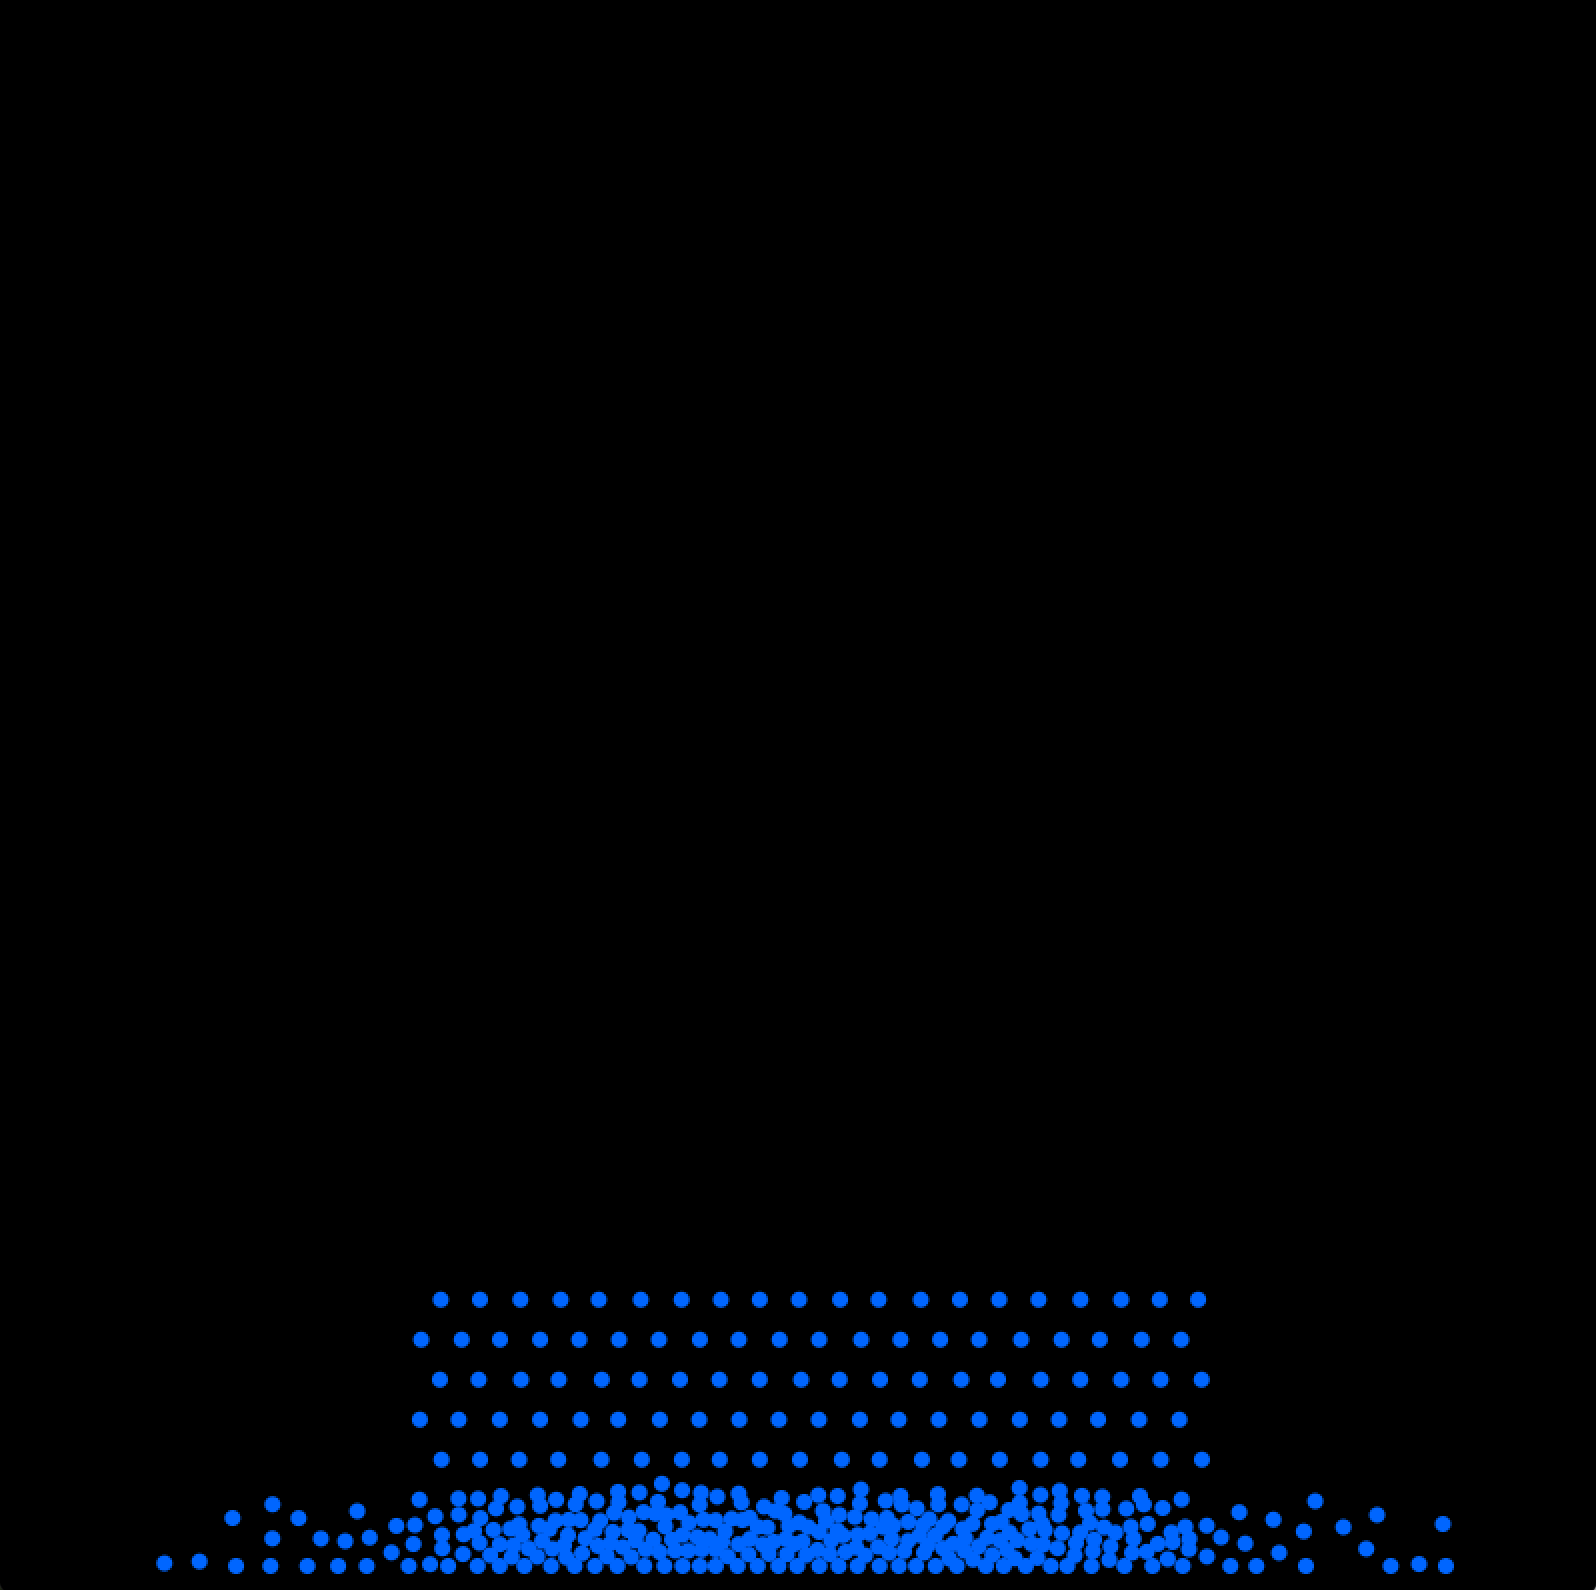
\includegraphics[width=\textwidth]{figures/particle400_2.png}
        \caption{first stage}
    \end{subfigure}
    \hspace{1em}
    \begin{subfigure}[b]{0.2\textwidth}
        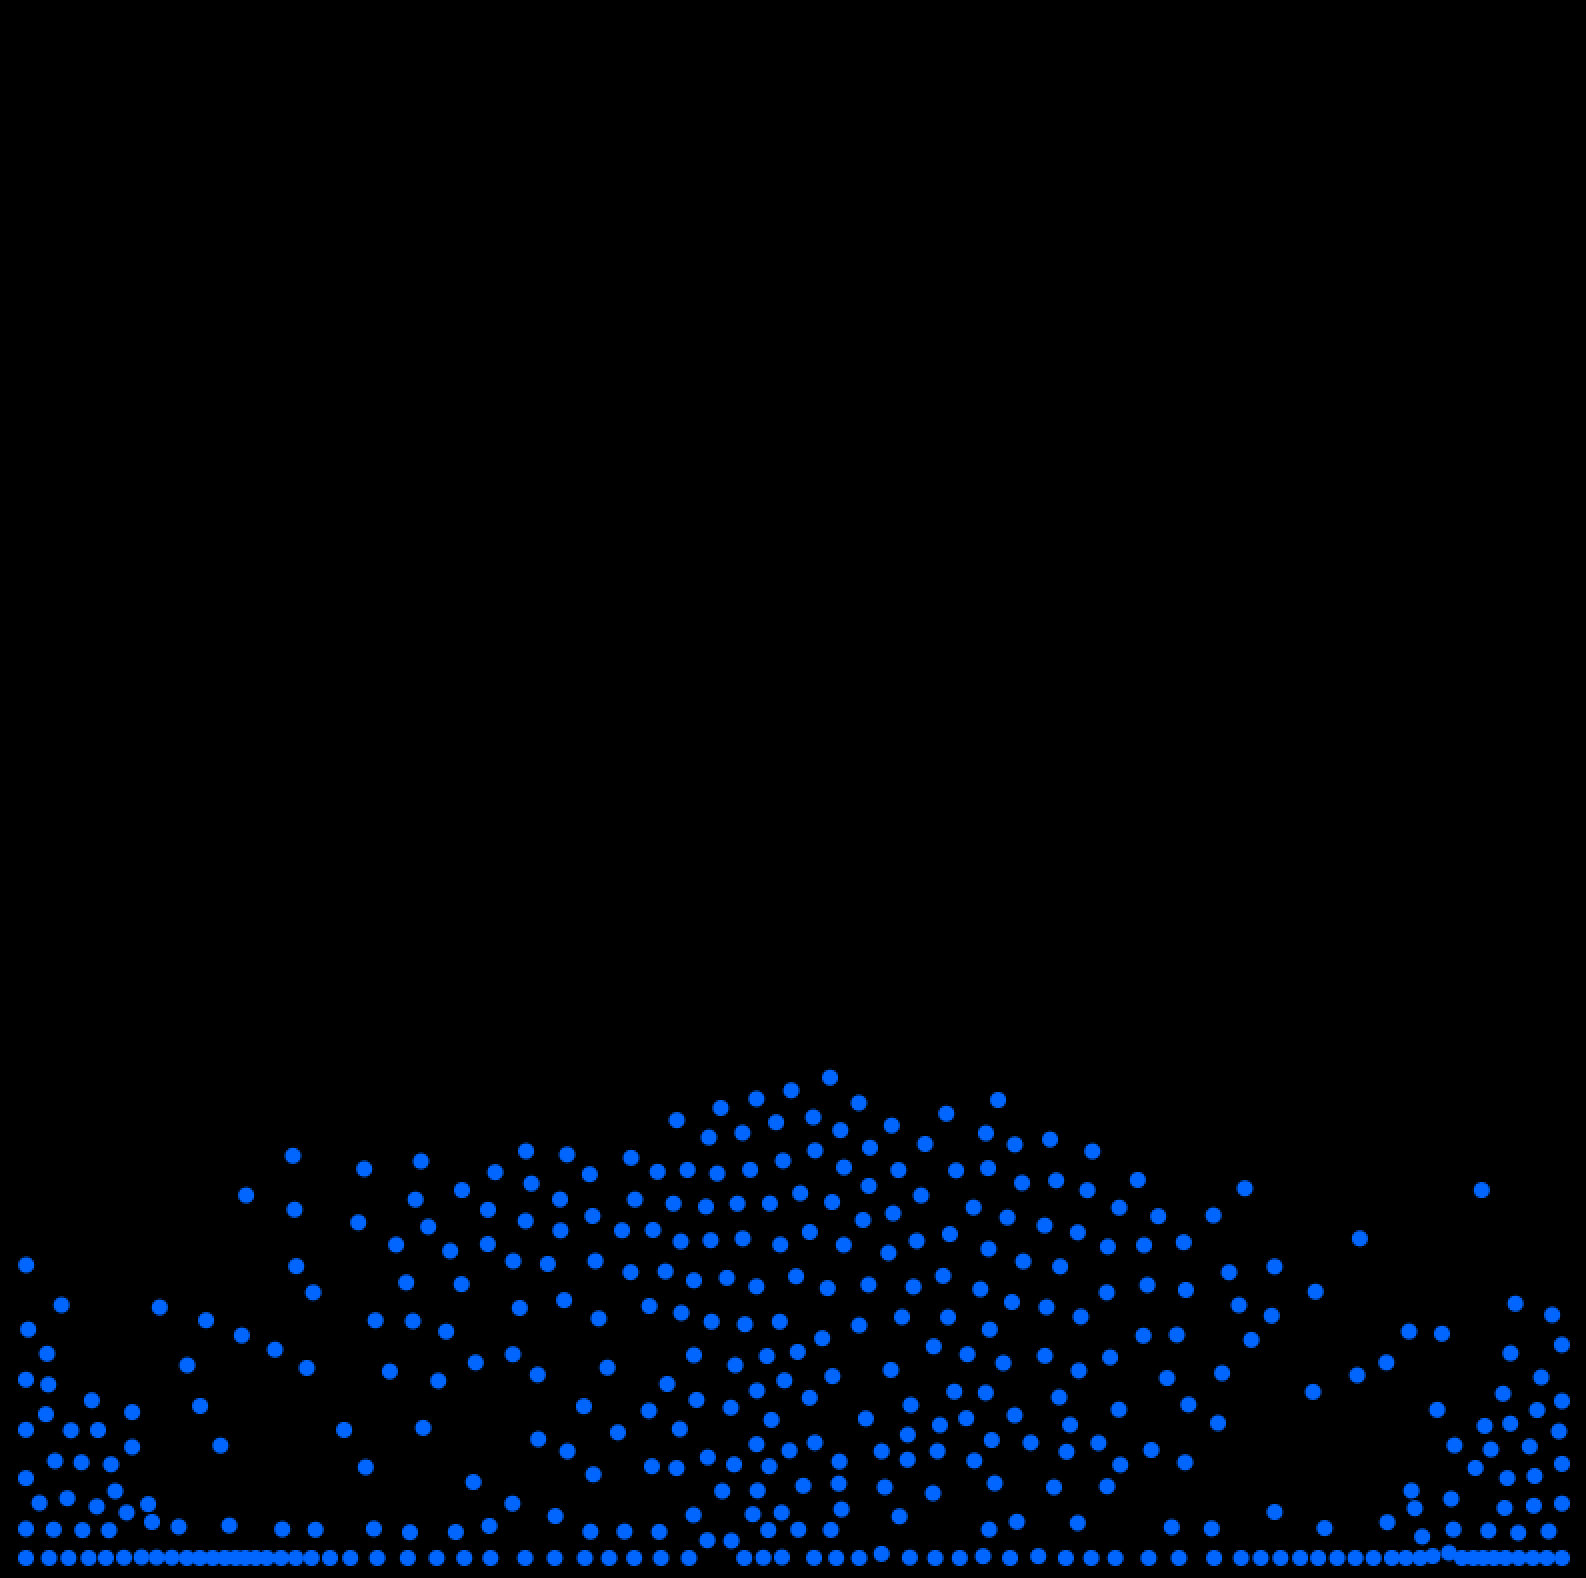
\includegraphics[width=\textwidth]{figures/particle400_3.png}
        \caption{second stage}
    \end{subfigure}
    \hspace{1em}
    \begin{subfigure}[b]{0.2\textwidth}
        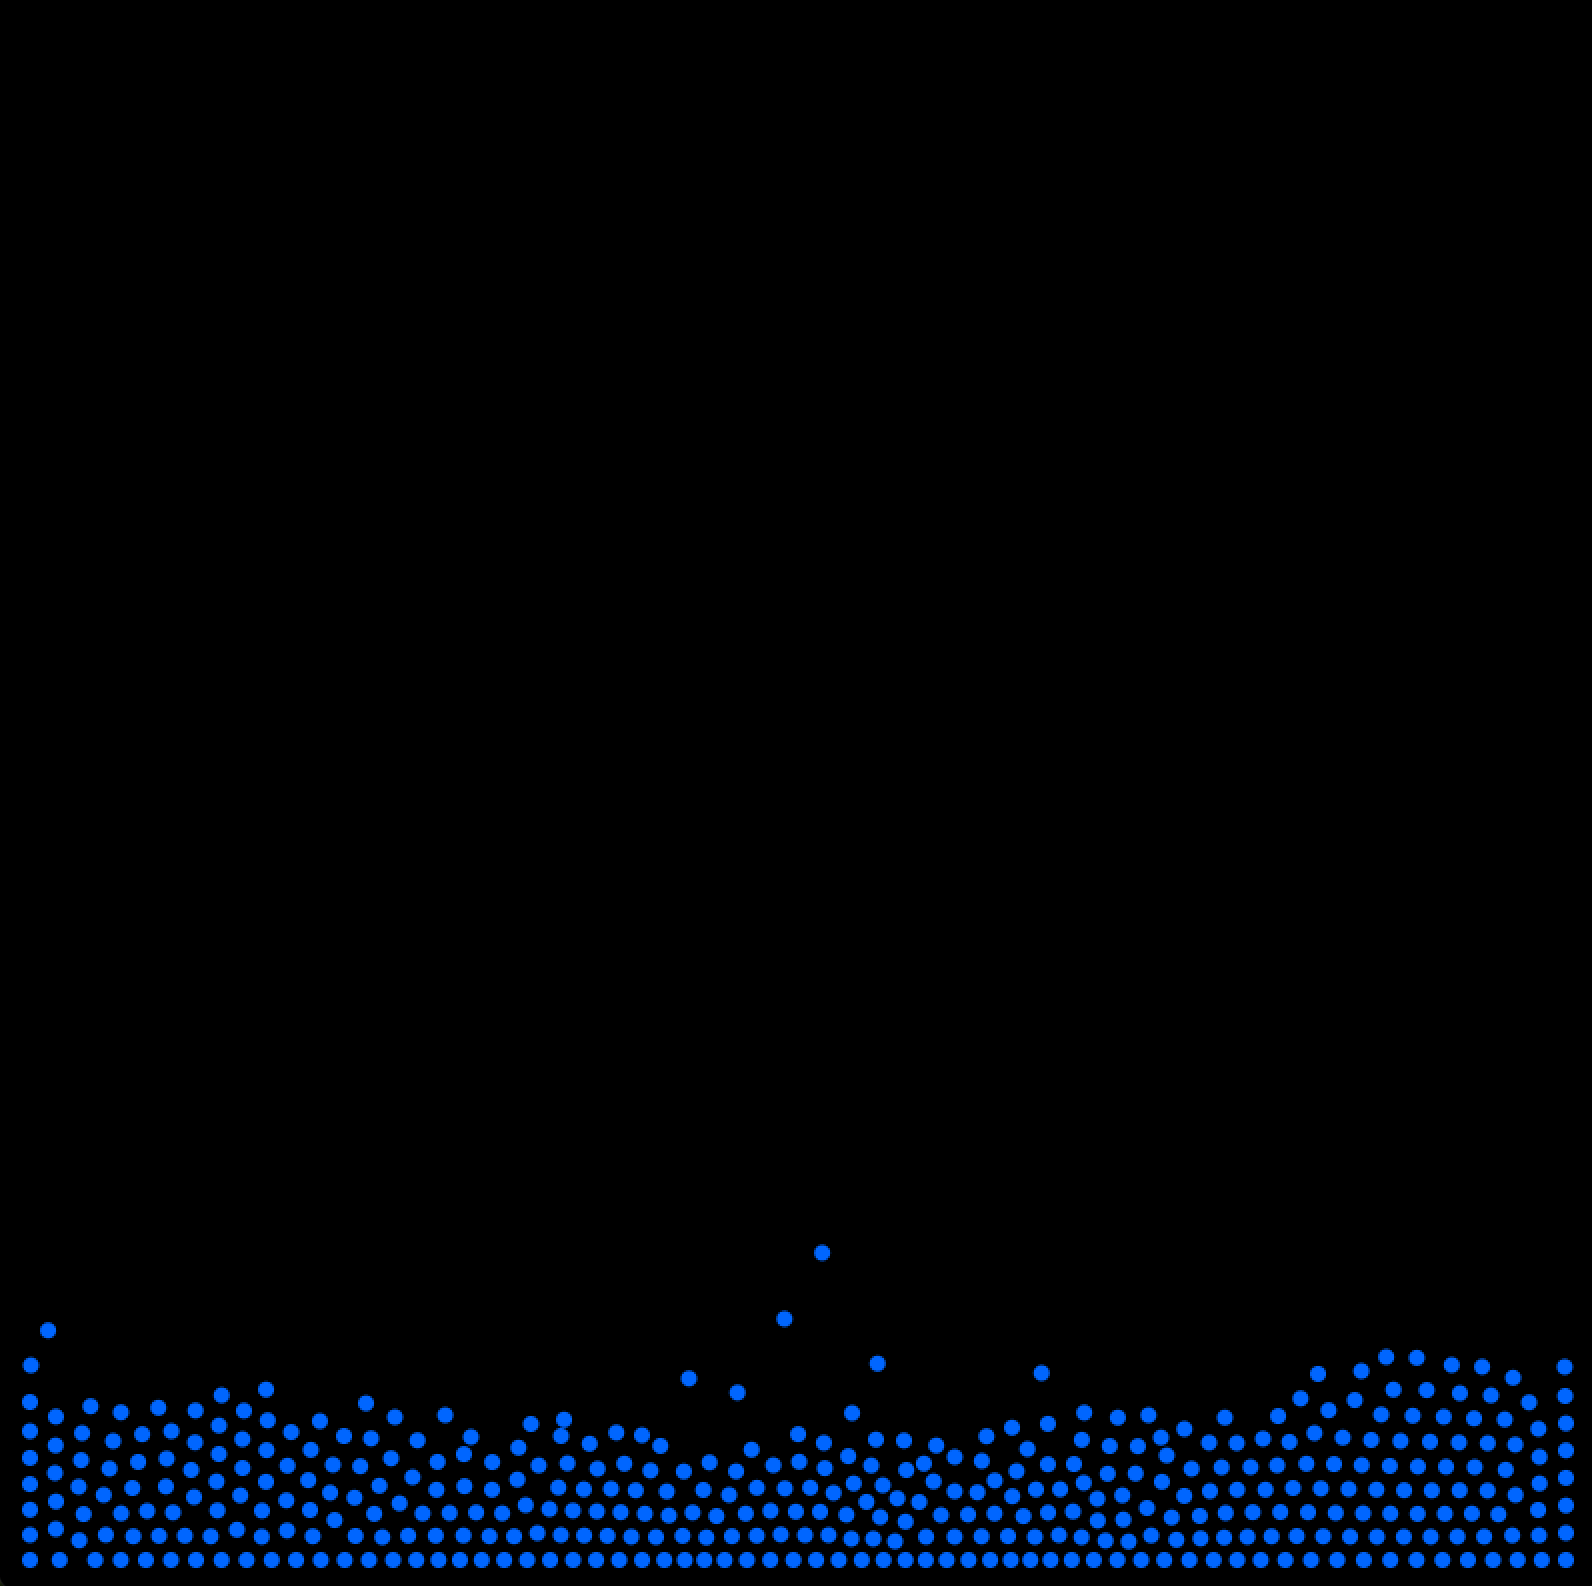
\includegraphics[width=\textwidth]{figures/particle400_4.png}
        \caption{third stage}
    \end{subfigure}
    \caption{
        Stages of Smoothed Particle Hydrodynamics simulation with 400 particles.
        (a) shows the initial particle configuration.
        (b)–(d) show the fluid evolution over time.
        SPH handles free-surface motion intuitively, but stability decreases compared to grid-based methods.
        }
    \label{fig:sph}
\end{figure*}

\subsection{PIC and PIC/FLIP}

We tested both the PIC and PIC/FLIP methods with the same number of particles. Figure~\ref{fig:pic_comparison} shows how the motion is more dynamic than pure PIC.

The PIC method loses energy fast. Particles move less and quickly fall to the bottom.
The PIC/FLIP method keeps more energy. Particles move more and look more natural.

\begin{figure*}[h]
    \centering
    \begin{subfigure}[t]{0.2\textwidth}
        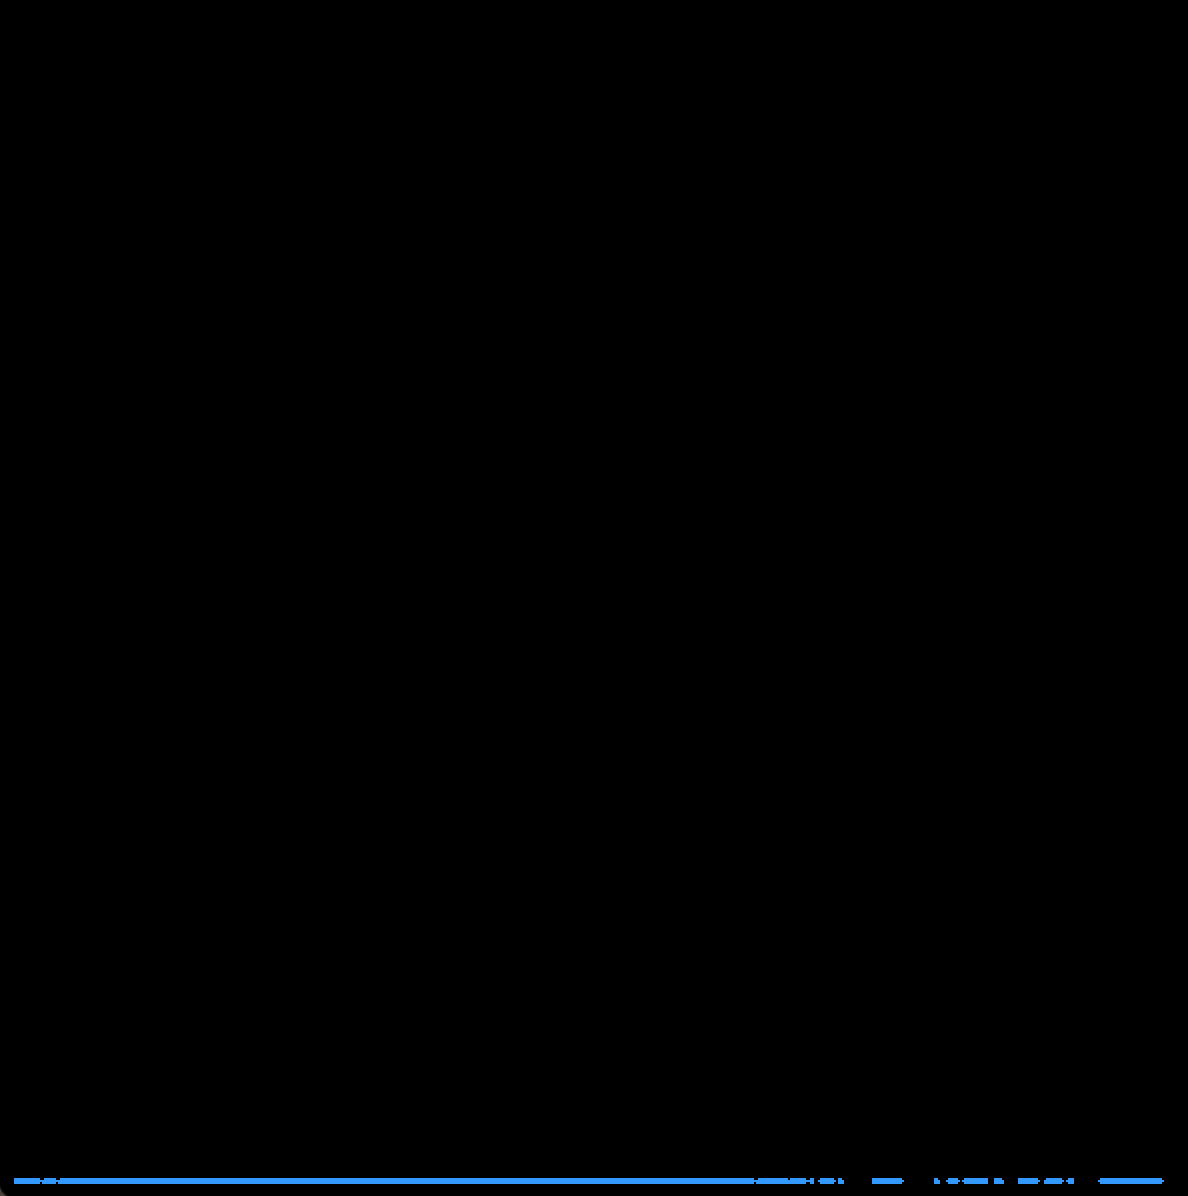
\includegraphics[width=\textwidth]{figures/pic_result.png}
        \caption{PIC result: motion is more damped.}
    \end{subfigure}
    \hspace{1em}
    \begin{subfigure}[t]{0.2\textwidth}
        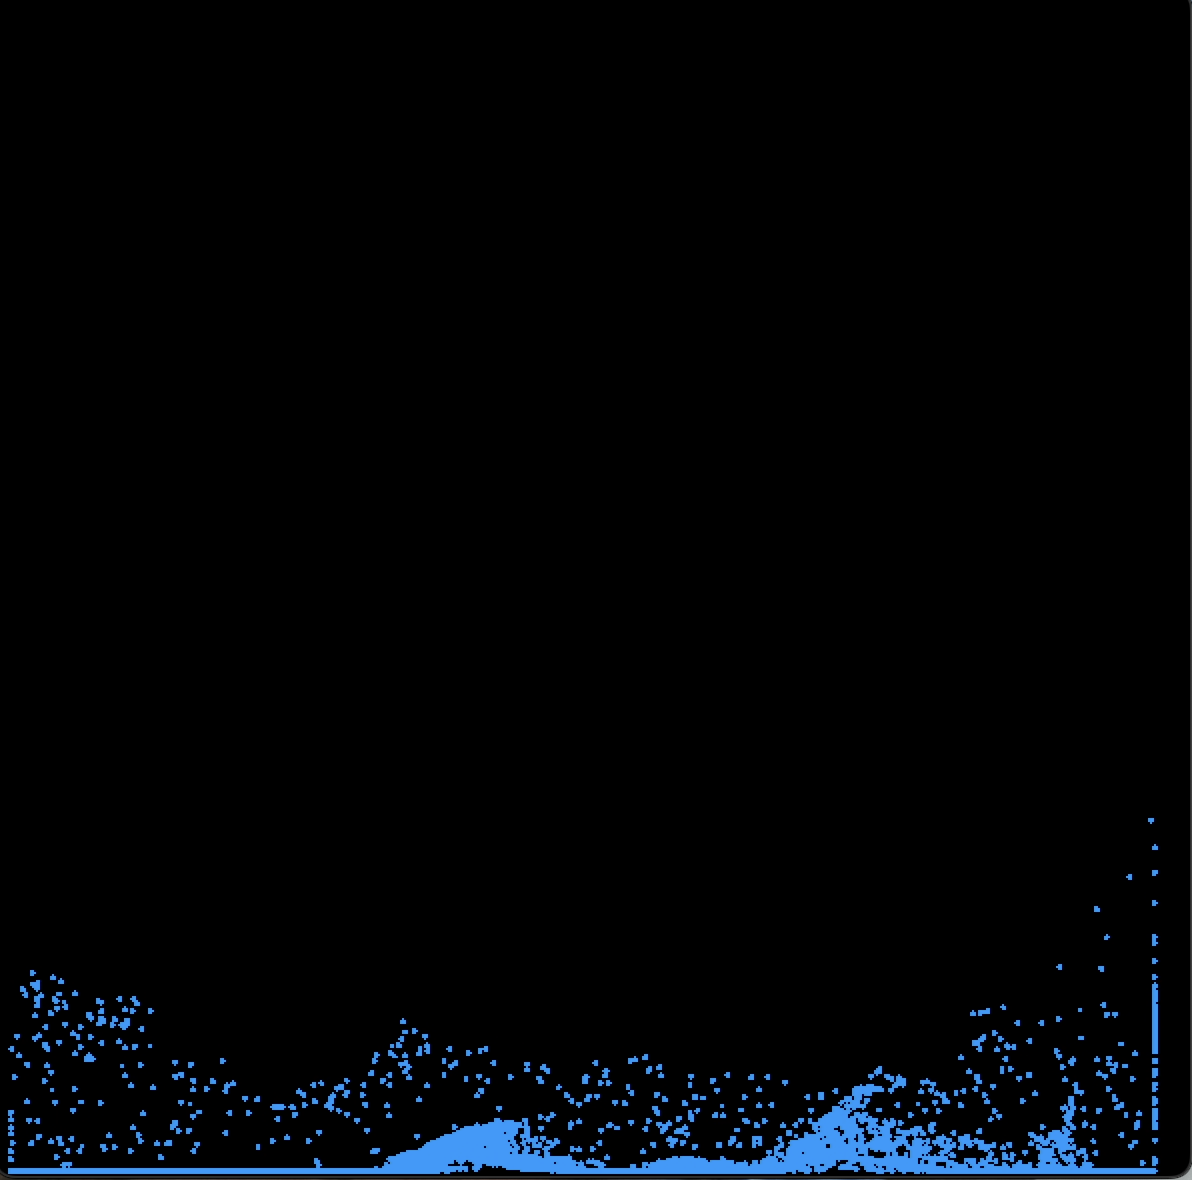
\includegraphics[width=\textwidth]{figures/pic_flip_result.png}
        \caption{PIC/FLIP result: motion is more dynamic.}
    \end{subfigure}
    \hspace{1em}
    \begin{subfigure}[t]{0.2\textwidth}
        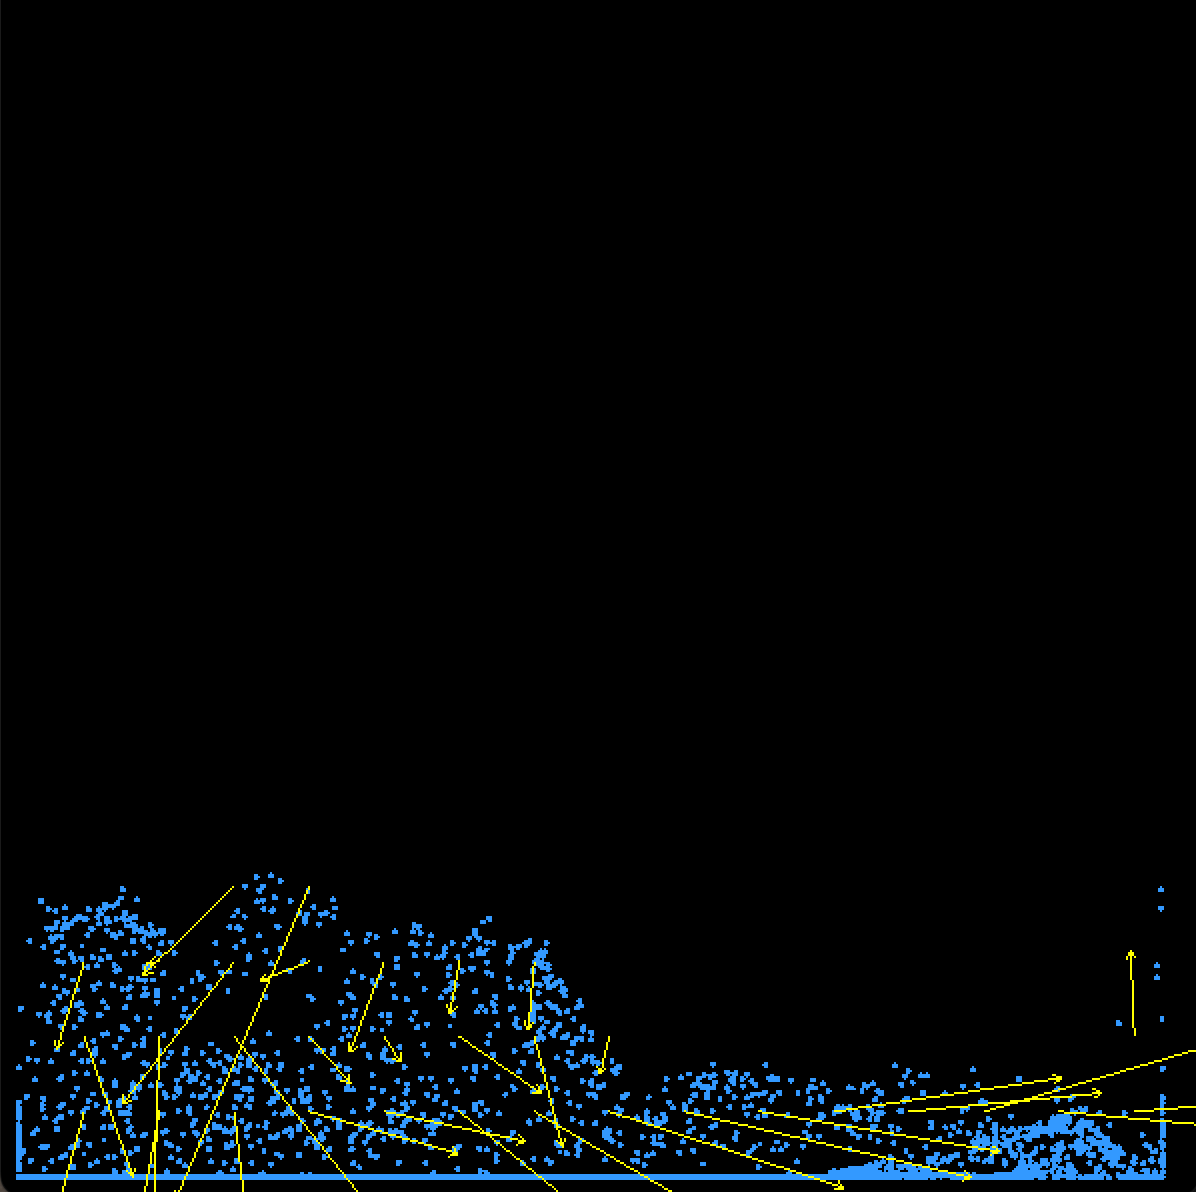
\includegraphics[width=\textwidth]{figures/pic_flip_interm.png}
        \caption{Grid velocities of PIC/FLIP}
    \end{subfigure}
    \caption{Final particle positions using PIC and PIC/FLIP. Both start from the same initial state, but show different behavior due to how velocity is transferred.}
    \label{fig:pic_comparison}
\end{figure*}

\subsection{APIC}

The APIC method produced the highest visual quality among all methods tested. By assigning each particle an affine velocity matrix, APIC preserves both rotational motion and local deformation, resulting in smooth and detailed fluid behavior. It outperforms PIC and FLIP in maintaining coherence and reducing numerical dissipation or clumping, especially at higher particle counts.

However, APIC is computationally expensive due to matrix operations and additional interpolation. Performance starts to degrade above 10000 particles, and implementation is more complex compared to PIC or FLIP.

We tested APIC with varying particle counts. Figure~\ref{fig:apic_comparison} shows snapshots at 1000, 4000, and 8000 particles. As particle count increases, the fluid becomes smoother and more realistic. The affine velocity transfer helps preserve structure during motion and reduces artificial viscosity commonly seen in simpler methods.
\begin{figure*}[h]
    \centering
    \begin{subfigure}[b]{0.2\textwidth}
        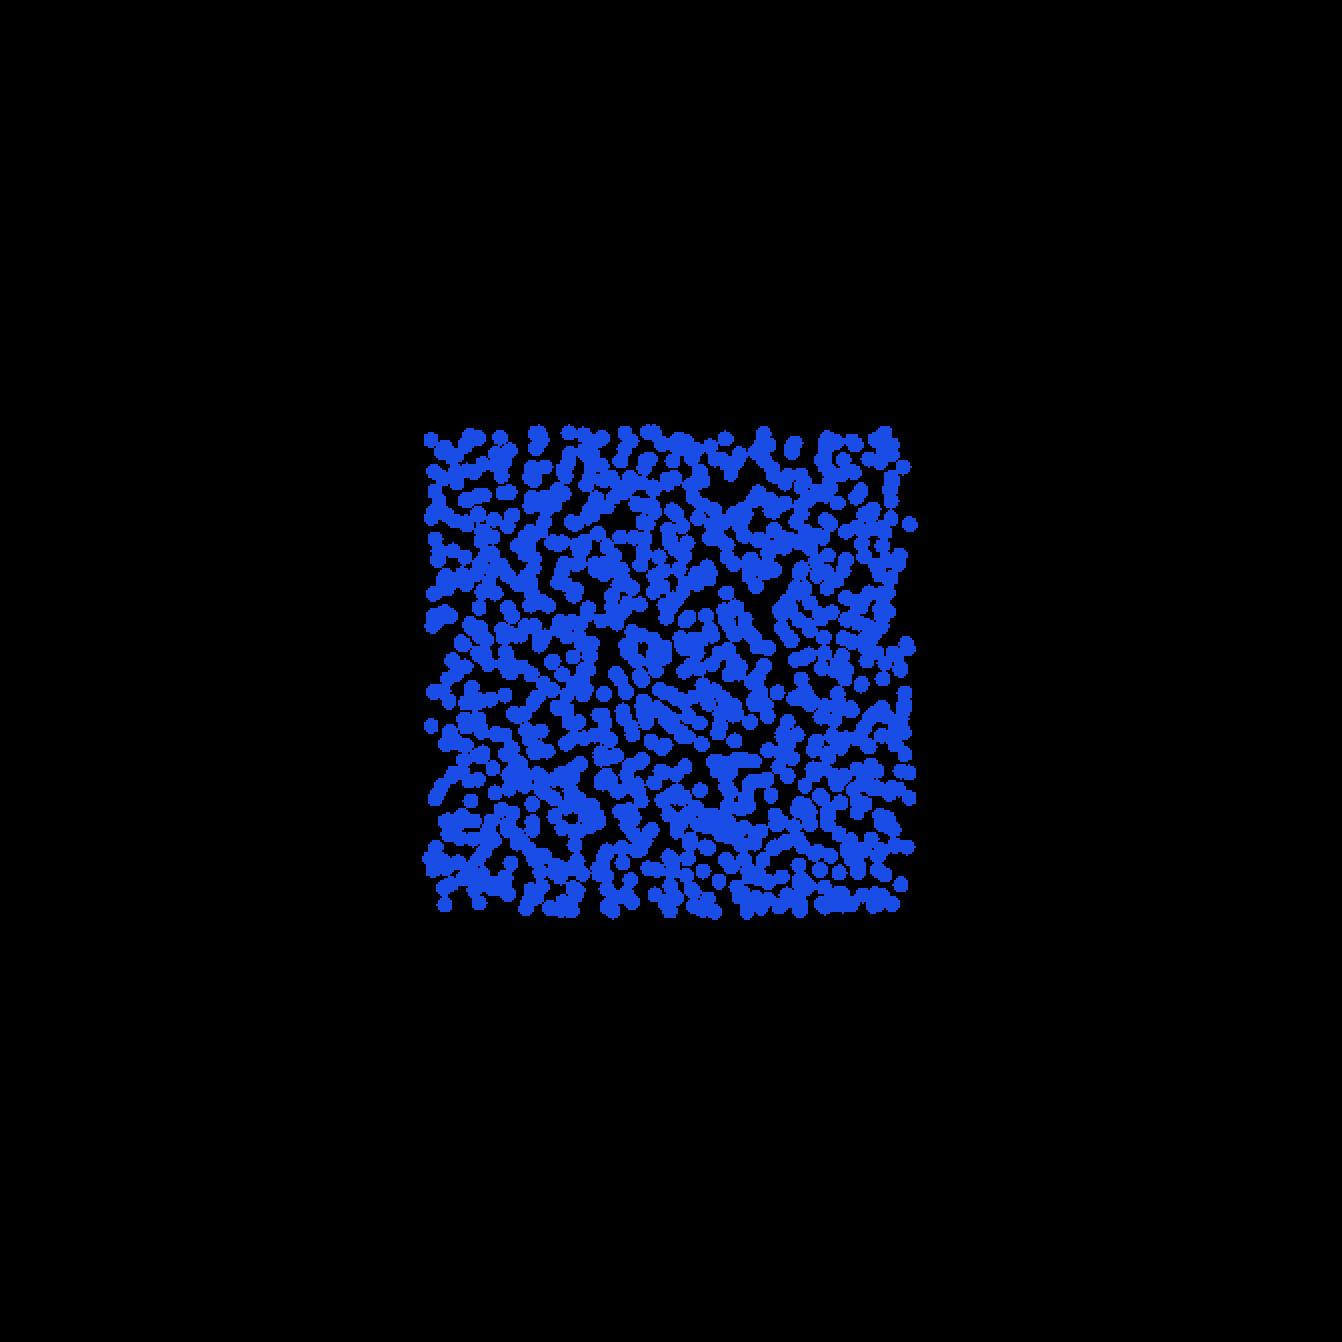
\includegraphics[width=\textwidth]{figures/apic1000_init.png}
        \caption{1000 initial particles}
    \end{subfigure}
    \hspace{1em}
    \begin{subfigure}[b]{0.2\textwidth}
        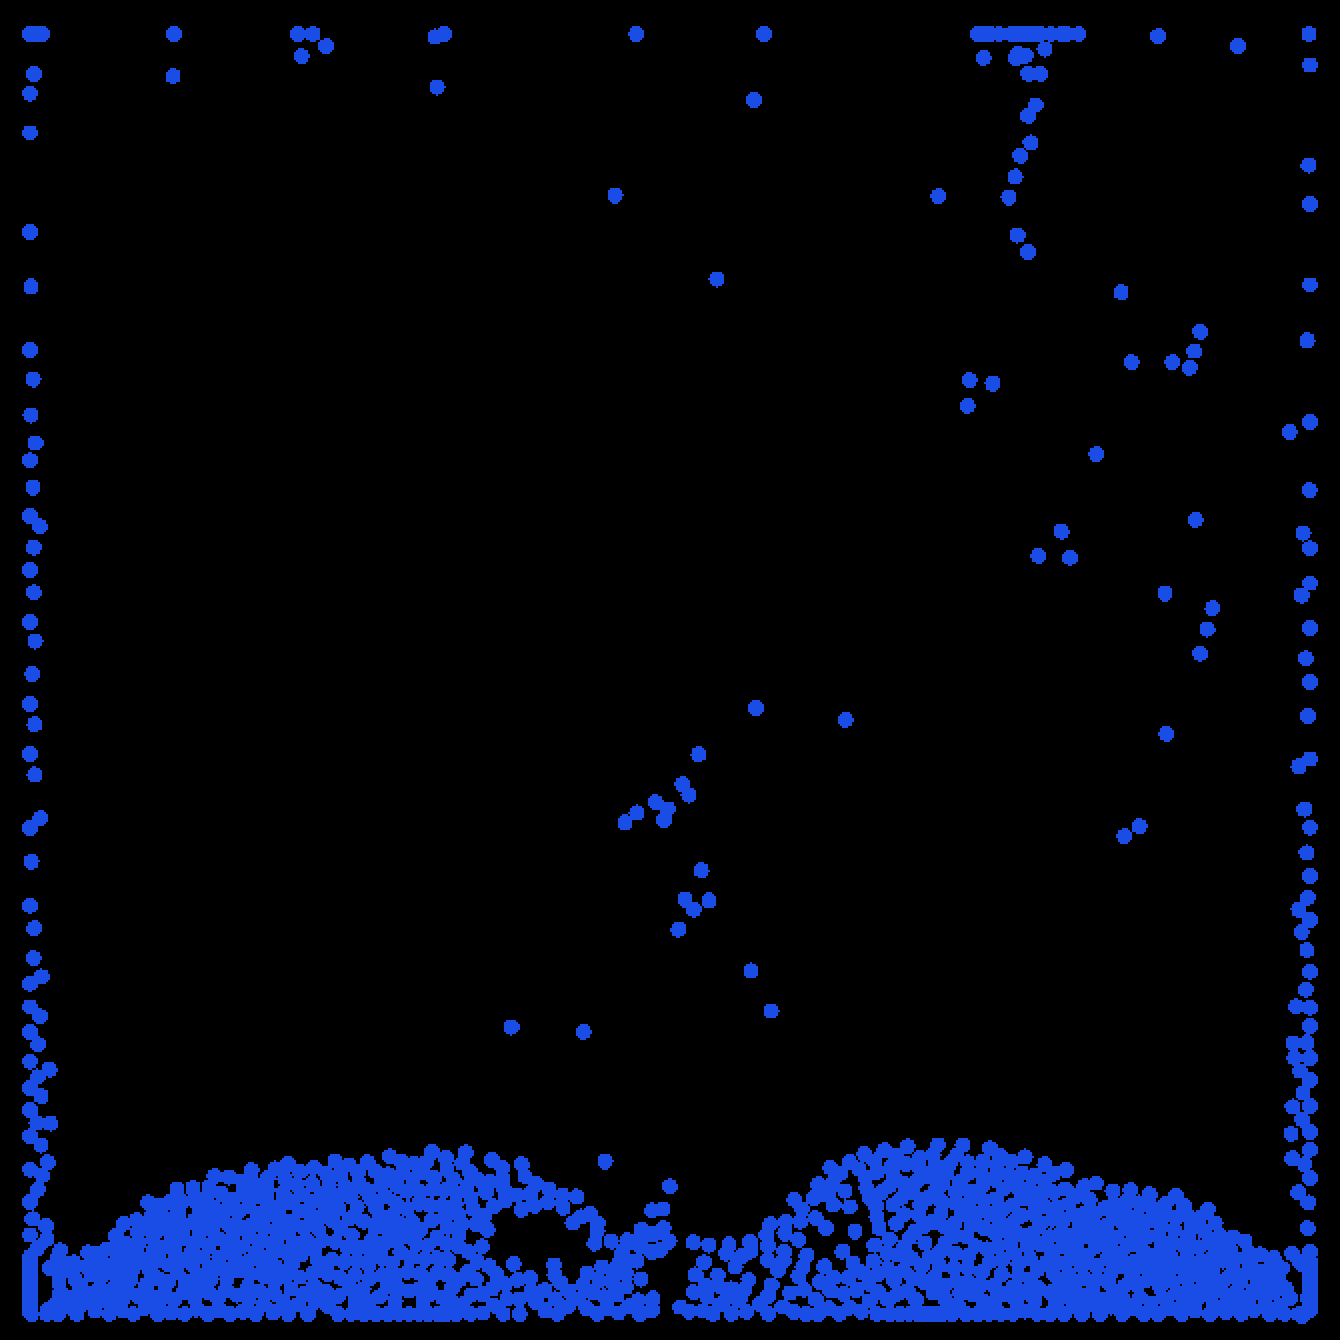
\includegraphics[width=\textwidth]{figures/apic1000.png}
        \caption{1000 particles}
    \end{subfigure}
    \hspace{1em}
    \begin{subfigure}[b]{0.2\textwidth}
        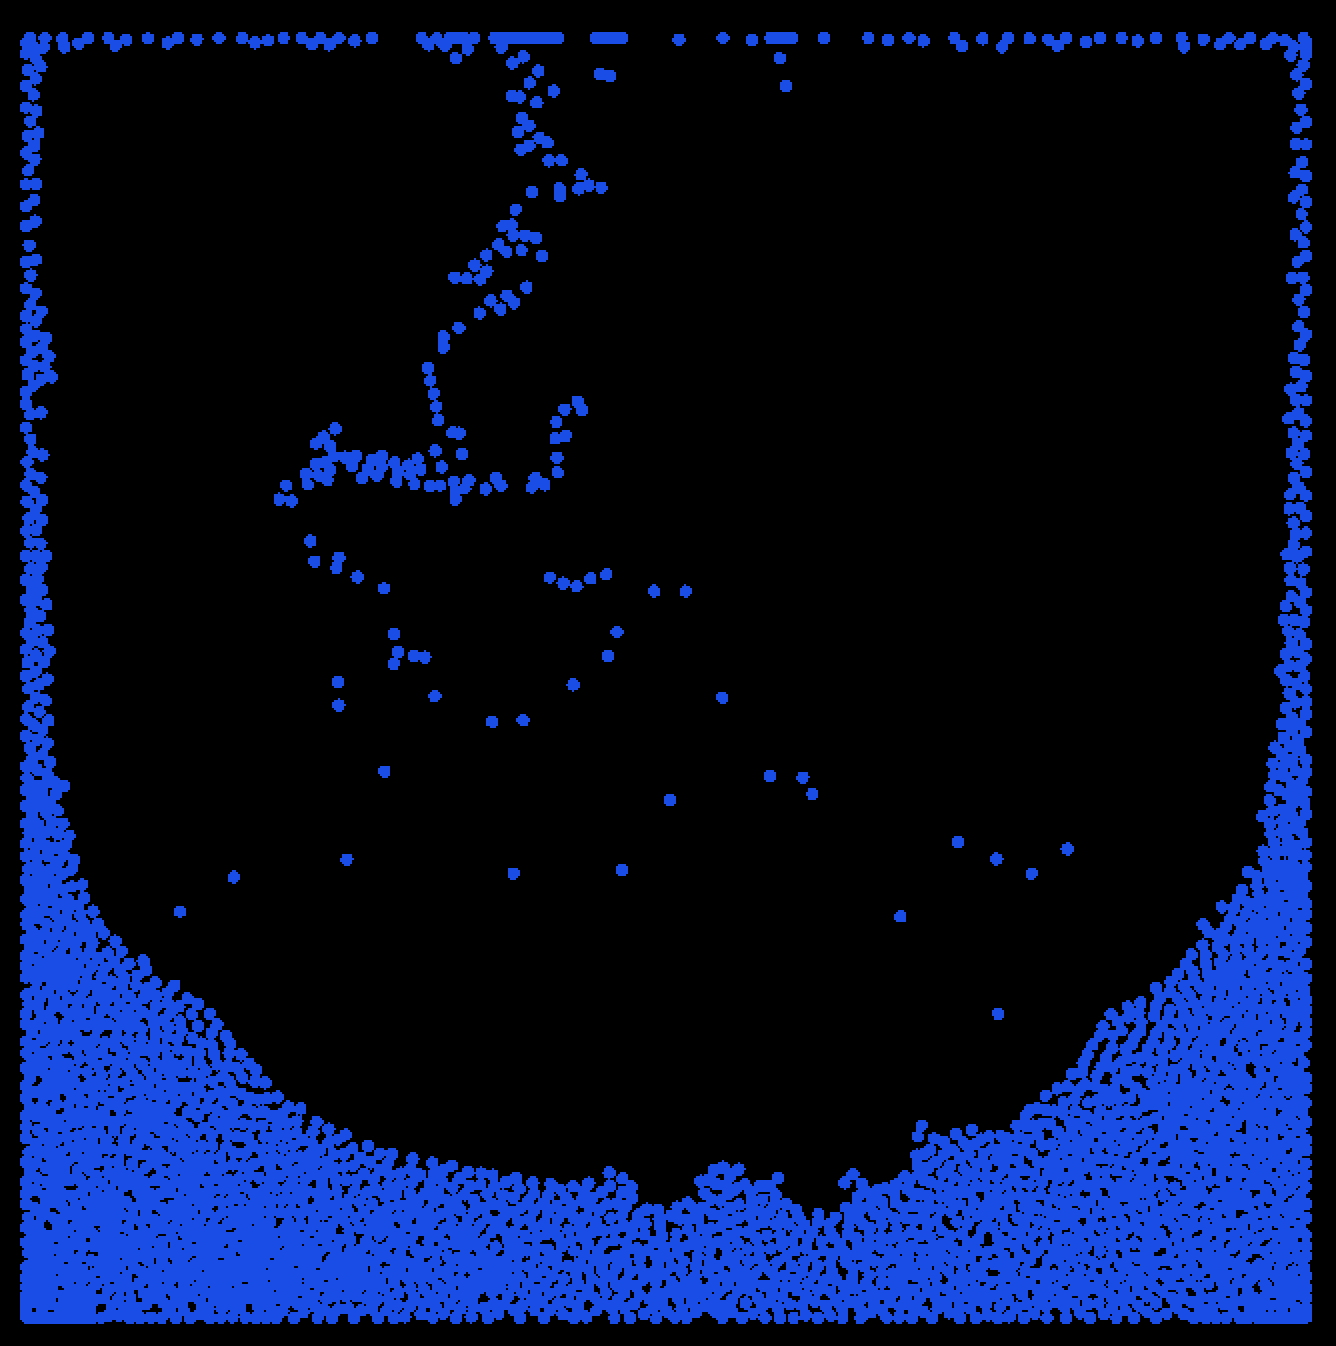
\includegraphics[width=\textwidth]{figures/apic4000.png}
        \caption{4000 particles}
    \end{subfigure}
    \hspace{1em}
    \begin{subfigure}[b]{0.2\textwidth}
        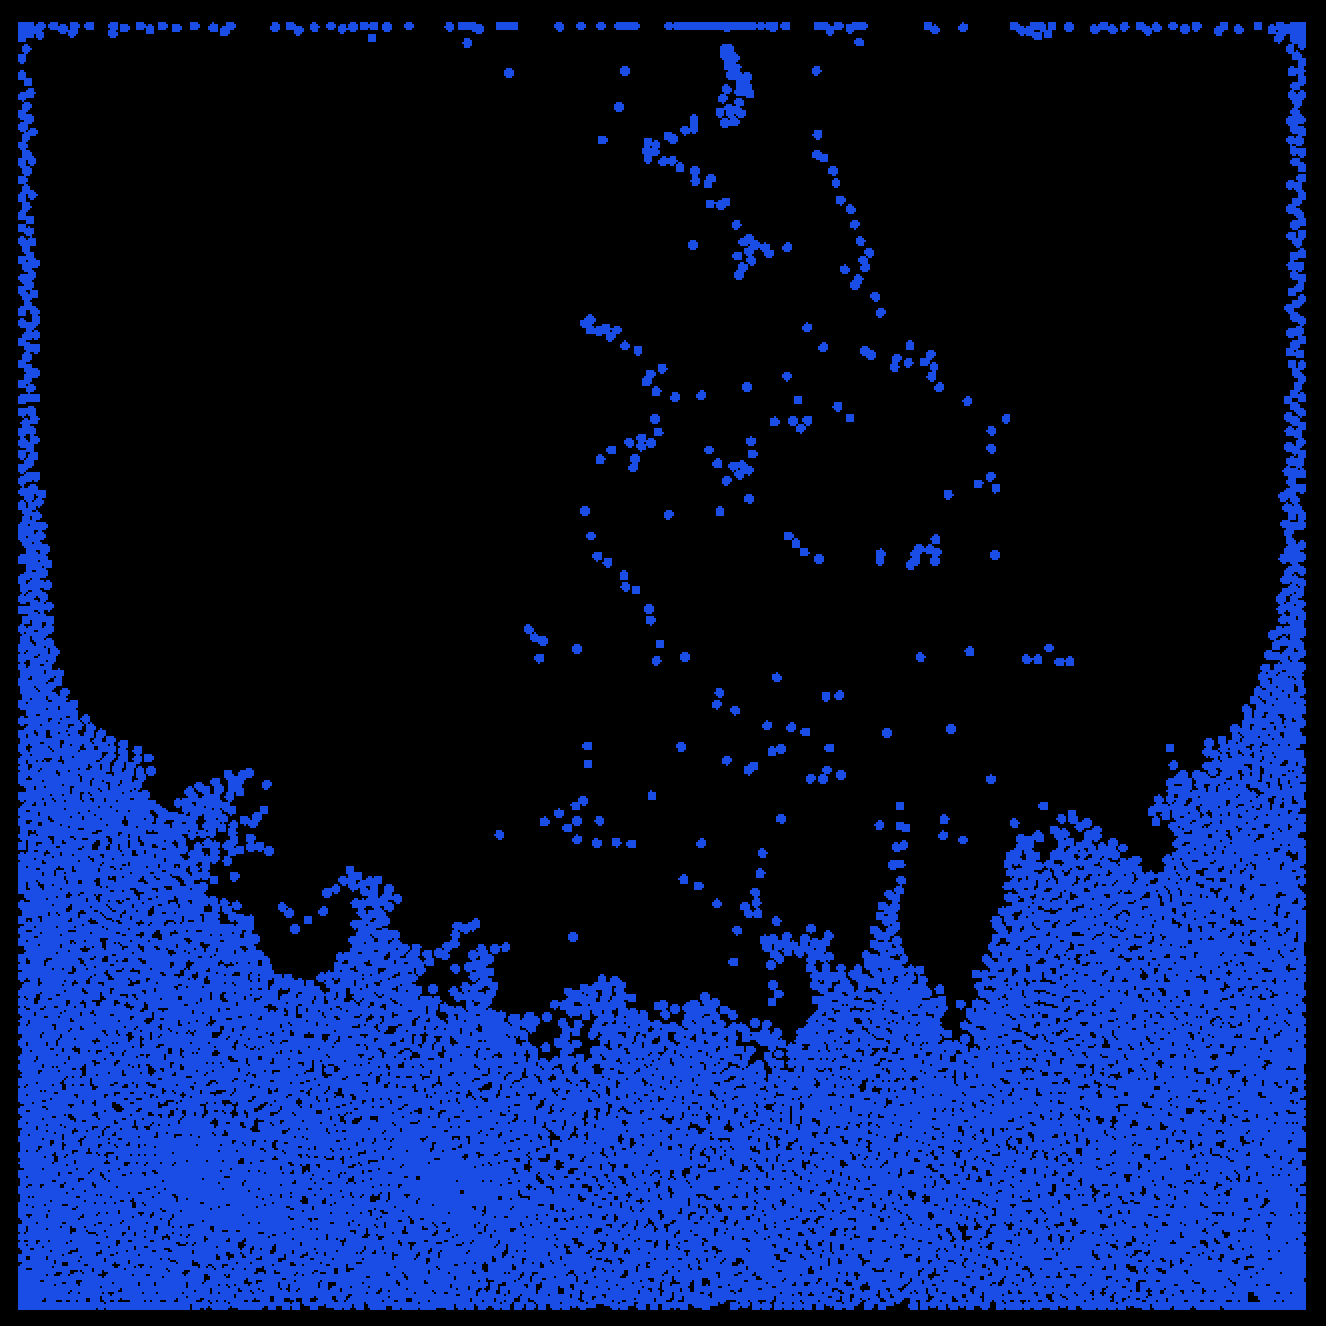
\includegraphics[width=\textwidth]{figures/apic8000.png}
        \caption{8000 particles}
    \end{subfigure}
    \caption{Comparison of APIC simulation results with increasing particle counts. 
    (a) shows the initial particle configuration, where all particles are placed in the center of the domain. 
    (b)–(d) show the simulation at the moment particles start to fall under gravity.}
    \label{fig:apic_comparison}
\end{figure*}


